%!TEX root = ../../report.tex

 
\section{Technical}

% 0.5 page
\subsection{Introduction}
As a part of the VSD framework, a technical part of the recommender system is required. In this chapter of the report, a focus will therefore be on the actual domain where the system is to be implemented, the technological choices taken for the systems. This will be done with the chosen values from the conceptual section in mind and grounded in these values. 
The section are divided in to two parts. The first will be an analysis, whereas the second will focus upon the implementation and challenges for doing so. 
A recommender system can be seen in many forms and be found many places, as described in section \todo{ref til section}. For this report, a recommender system for courses at the IT University, will be conceived. The reason for this, is that all full-time students are faced with one or more options for non-mandatory courses throughout their education. This can, for some students, be hard to do, because of the many courses available as well as the lack of transparency of the content for each of these courses.\\

The intuition for the system can be divided in to three basic step. The first is some sort of data extraction from the systems at ITU, that holds the data needed to make a recommendation. The second step is to prioritize this data and select only the relevant. The third step is to process the selected data and transform this into some sort of structure holding students and courses and thereby constructing the recommendations for every student.


% 0.5-1 page
\subsection{Domain Description}
In order to design the system it is needed to explore the domain in which the system needs to be designed. To get an overview of this, this section will be used to explain the different terms which is used and explanation of what kind of educations the university offers students. Some works used here will be domain specific, but will be explained in the Glossary found in Appendix \todo{REF TIL GLOSSARY}
To start at the highest level, the educations is divided into 3 sections: Bachelor, Master and Diploma. Both the Bachelor and Master are full time studies, whereas the Diploma is targeted for people already working and wants to complement or upgrade their education. There is three types of bachelors tracks: Global Business Informatics (BGBI), Software Development (BSWU) and Digital Media and Design (BDMD). The Masters are divided into: Digital Innovation \& Management, Digital Design \& Communication, Software Development and Technology and lastly Games. Under the Masters different tracks (also called specializations) can be chosen, but these will most likely not be taken into considerations in the system, and therefore not explained here. The Diploma is designed to be a part time education, with single elective courses. Also here, it is possible to choose tracks, but like the Masters, will these not be explained. 
A bachelor education consists of 180 ECTS points, a Master on 120 ECTS points and Diploma 60 ECTS points. Since the Bachelors consists of many mandatory courses, not a lot of ECTS points a available for elective courses. The direct opposite is the case for the Masters. Here most of the 120 ECTS points are elective, which is the same for the Diploma. 
The different people associated with ITU can be divided into three groups: Students, Researchers and Staff. The most interesting group is of course the students, since this in this group, the recommendations will be targeted. This group can be further divided into full- and part-time students. Most people on the Bachelors and Masters are full-time whereas a small part of Masters aswell as all people on Diploma are part-time, for different reasons. 
The three types of educations all have elective courses, but the the Masters have more 
COURSES?
What domain are we in? Description of special words. Explanation of the different educations/track/etc

% 1-2 page
\subsection{Design Choices}
In this section explanations of the design choices made throughout the design process will be presented aswell as the 'consequences' of choosing the different solutions. 
\subsubsection*{Collaborative or Content}
One of the first and most important choices made for this system, is of course what kind of recommendation type of system, that should be developed. In section \ref{chap:chapter1} we outlined three different types of recommender systems: Collaborative-filtering (CF), Content-based (CT) and Hybrid approaches. As also explained in \ref{sec:collaborative} and \ref{sec:content} the two first types somewhat represents extremes and it is most common to use a hybrid of the two. To keep the system as simple as possible for a start, the approach chosen is the content-based one. The reasons for this, will be outlined below. \\
The CF approach mostly builds upon ratings from users, which is used to either compare users with users or items with items, and then produce a list of recommendations. This makes the ratings a central and crucial part of the system. In order to implement this approach for a ITU recommender systems, these ratings could come from the course evaluation, which basically asks the students to 'rate' and comment on both the course and teacher. This could definitely be a viable solution, except that it relies a great deal upon the data from the course evaluation. Unfortunately the evaluation is only done by around 35-40\% students, which means the system will be affected of the things described as the 'Data sparsity' problem in section \ref{subsec:data_sparsity}. Even though many recommender systems suffer from this problems \todo{kilde?}, and are still implemented, the other approach have been chosen. Another problem would be the reliability of the ratings. Even though these would come from the students, and thereby represent their opinion about the courses, the would properly more reflect how popular are course are, more than the actual content of each course.\\ 
The primary reason for choosing the CT approach is the availability of keyword for each course. Each of the courses available for the students, has an associated course description, which will be the primary source of content. In contrast to the CF approach, using the keywords from the course description, instead of ratings, would represent what the teacher thinks and imagines about the course, which is a more authentic and representative source of information. 

NOTE: A key thing to note here are the distinguishing between the popularity of a course (rating) and the content of a course (keyword).

\subsubsection{Persistent or memory?}
\label{subsec:persistent}
As part of the design process, it is necessary to look at the usage of the system, in order to choose if data should be read into memory at run-time when needed or a more persistent choice of data storage is needed. The answer to a question like this is closely related to when and how often the system is running. If the recommendations are needed many times daily or weekly, the choice would be to have the system running on a server, with a database taking routines backup of things like the different users profiles and recommendations. If the the system only would run a couple of times a month or year, one option would be to load all the raw data into the system for each run. Even if this process would be expensive to perform, it is easy to argument this being okay, since the data would only be used a few times and could be loaded in before actually needing it. Another option would be to load the raw data into the system on the first run, stripping it for unecessary information and then storing this data in a database and then just only update this database with new data, before each run. This latter option have been the chosen solution, since it enables the system to spend less time reprofiling all students for each run. It is only necessary to profile new students and courses. This should in theory reduce the time needed to calculating the recommendations.

NOTES:
even though the program only will run 2-3 times per year, perstiente the data to a database is needed. One could simpy keep the data in memory, but then it would be needed to 'reprofile' all students and analyse the content for each course, for each run of the program. When persisting the data, the program 'only' needs to compare the new data with the previous created profiles and the content for the courses.


Target group?
Tidsplan?
% 0.5-1 page
\subsection{Data Modeling}
Following the section \ref{subsec:persistent} a analysis of the data for ITU, including information about students and courses, was needed. This analysis are then devised into a model of data, which we have chosen to represent using a ER-diagram. This is useful for further discussions and improvement of the system, but can also serve as inspiration for the classes and objects needed at the programmatic abstraction layer. 

\subsubsection{ER-Diagram}
The ER-diagram following below reflects our considerations and reflections about how to represent the selected data in relational database. At the time of writing, where no real implementation has taken place, this diagram reflects the bare minimum required for the development of the system. The reason for not including the rest, is that this is best done with a agile and iterative development process, which have not been possible to engage in due to a time-constraint. It represents the results of the data selection process, which have been about prioritizing the available data from ITU in to the relevant data for the system, which have meant we have excluded some non-needed information attributes.

\begin{figure}[H]
\centering
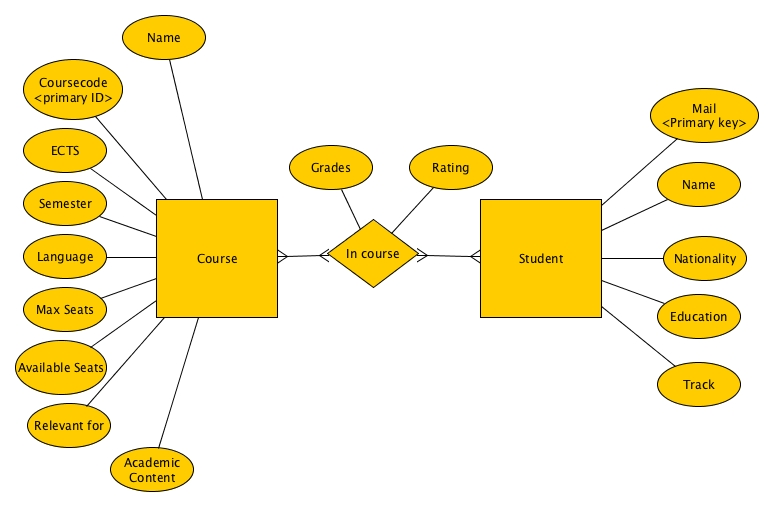
\includegraphics[scale=0.5]{Pictures/ER-Diagram.jpg}
\label{ER-diagram}
\caption{ER-Diagram}
\end{figure}

% 0.5-1 page
\subsection{Architecture Analysis}
Flow of the program
Picture of package diagram/components

% ? page
\subsection{Glossary}
\begin{itemize}
	\item[ECTS points] 
	\item[SWU]
	\item[GBI]
	\item \todo{more?}
	\item[CF] Collaborative-Filtering approach
	\item[CT] Content-based approach
	\item[Course evaluation]
\end{itemize}
% 1-2 page
\subsection{ITU Recommender System}
So far the previous sections have described the domain and the surrending parts of the actual system. In this section, we will go in to depth with the actual recommender system and its individual components. The responsibility aswell as the input and output will be decribed for each components. The the order of this section follows the flow of the program and will therefore start med the Content Analyzer.
\subsubsection{Content analyzer}
This component are responbile for analyzing all courses available at ITU and construct a vector for each of these courses. The input of courses, will come from the Data Processing \todo{Describe Data processor} and the output will be a in some sort of abstract data type, possibly like a map. The process of producing the vectors are expressed as the pseodu algorithm below:
\begin{itemize}
	\item Make a list of non-keywords like "this", "and", "is" or "will". (\todo{NOTE}: This will cause the system to be less biased (fairness?), compared to a humar (Rune) selecting the keywords.)
	\item Construct regex which identifies ALL words in the current document, except the ones from the non-keyword list
	\item Count number of occurrences of each word found by the regex expression
	\item Repeat step 2 and 3 for ALL courses and construct a datastructure of maps with maps. Meaning the first map has the course code as key and the value being a map containing each specific keyword and key and the number of occurences as value. 
	\item Use the TFIDF \todo{Ref to TDIFD formula} formula for each course, which will produce a vector space containing n-keywords dimensions, where each dimension contains a vector with a lenght representing the weight of this keyword, for this specific course 
	\item Use the Cosine normalization formula for normalizing every keyword vector for all courses.
\end{itemize}
At the end of this algorithm, each course will have an associated vector, which represents the value, in relation to keywords, of the course compared to all other courses. The resulting data structure, will then be used by the Filtering Component and the Profile Learner, which will be described below.

\subsubsection{Profile Learner}
This component is used to analyze every student preferences. To do this, some feedback or history from the students are needed. This feedback will, as explained \todo{where is it explained?}, come from the previous elective courses, that the student have been signed up for. The reason for using this information, is the fact, that we believe that this is the most significant and reliable source of information. Like the Content Analyzer, the flow of this component are expressed in form of a pseudo algoritm outlined below:
\begin{itemize}
	\item Find all elective courses the student have been signed up for, retrieving it from the Content Analyzer.
	\item Of these courses, compute the average vector (adding the vectors together and divide by number of vectors) by projecting each of the vectors on each other. This resulting vector represents the users preferences, in relation to the elective courses the student have signed up for. 
\end{itemize}
This will 'collect' all the elective courses the student have been signed up for at produce a resulting vector, which expresses the students preferences. If the student have had no elective courses, the Profile Learner will notify the Filtering Component and this will decide how to proceed. 
\subsubsection{Filtering Component}
This component receive the results from the Content Analyzer and the Profile Learner, in order to produce the list of recommendations for each student. The input needed, are the courses with a associated vectors for the keywords and a vector representing the each students preferences, based on previous elective courses. It used this information in the way described below:
\begin{itemize}
	\item In the list of courses taken from the Content Analyzer, sort out all the courses the student already have been signed up for. (the student are not allowed to sign up for courses, he/she already have been signed up for - \todo{VALUE-NOTE-->}This makes the system a bit bias, since the student could have been signed up for a courses, but failed it. Cases like this, will be ignored by the system. If a student have failed a course, the student will know if he/she wants it again, which will be hard to know for the system)
	\item In the list of courses taken from Content Analyzer, sort out all courses that the student will have as mandatory courses in the future.
	\item Use the resulting vector produced in step 2, to compare every course from the Content Analyzer to produce the list of recommendations.
	\item Sort the list of recommendations, having the courses with the most similarity (closest to 1) with the resulting vector 
\end{itemize}

\subsubsection{Data on students}
First step is to divide up the students into the groups where they belong, using the first five student data points.

- Education
- Track
- Semester (Bachelor students can only choose an elective course on 4th and 5th semester) (Masters students can choose an elective course on each semester (4th is only their thesis))
- ECTS points earned
- Nationality

Only when the students have been divided up into groups is where the recommender system will go to work. By analyzing the next student data points the RS will recommend elective courses to the students in question.

(which courses has the student already had, (DO NOT TAKE COURSE AND EXAM DATES INTO CONSIDERATION (AMAZON DOES NOT DECIDE WHETHER SOMETHING IS TOO EXPENSIVE FOR ME OR WHETHER I NEED THAT, THAT IS UP TO THE INDIVIDUAL TO DECIDE, THE SAME APPLIES HERE)))

- Grades (only in relation to elective courses?)
- Previous grades (all courses are available to all students that meets the formal requirements) (just because you get a low grade on a previous course does not necessarily makes that person less interested in a course where that previous course is a pre-requisite)
- Previous courses (mandatory) and projects
- Previous elective courses (could be a sign of interest)
- Age (when you have been accepted to ITU you are in and can freely choose which courses you wish to attend no matter of age - we do not want to implement any bias into the system)
- Current courses (to make sure that the recommended elective course is not time wise placed on top of on of the mandatory courses)

The last two student data point serves as contact information (name is also used to refer to the above mentioned data points).
 
- Name
- Mail
- 

\subsubsection{Course information}

- Name
- ECTS (should be included, so a student with only 7,5 etcs available, will not be recommended courses with 15 etcs)
- Which semester
- Course code
- Course language
- Max seats
- Current number of taken seats
- Formal requirements (to vaguely defined in order to extract proper information)
- Course learning goals (not important)
- Academic content (this is here the keywords are extracted for the recommender system)
- Mandatory activities (not important)
- Exam forms (date and description) (the student must check if exam dates collide)
- Litterature (not important)
- Curricullum (not important)
- Course responsible/manager (not important)
- Relevant for (needs to properly defined, but is usefull)
- Time and place (it is the students responsible to check if courses collide)



\subsubsection{List of Requirements}
\begin{itemize}
	\item The list of possible courses for each student, must NOT contain mandatory courses or courses the student already have had.
	\item Der skelnes mellem tilmeldte og tidligere tilmeldte kurser, i forhold til bestået kurser, for at undgå at man bliver anbefalet kurser, som man er igang med på tidspunktet hvor anbefalingen falder. 
\end{itemize}
  

\subsubsection{Recommender system output}

- Max seats in recommended course
- Current number of seats taken in recommended course
- NOTE: please check that the recommended courses are not colliding with your mandatory or other elective courses
- 




FIND INFORMATION THAT DESCRIBES HOW A CONTENT ANALYZER, PROFILE LEARNER AND FILTERING COMPONENT ARE 

MAKE NEW DRAWING SHOWING THE INFORMATION FLOW WITHIN THE SYSTEM BOTH FOR CONTENT-BASED AND COLLABORATIVE



IF COLLABORATIVE BASED (ALWAYS RATING BASED): USER-USER OR ITEM-ITEM

It will be a choice between what the course contain (can't really be shown from the users ratings of the course, since two courses can be completely different in regard to content, but have the same overall ratings) and how popular the course is (can be shown by the ratings, but will be a problem with new courses). Only about 40 percent of students are rating their courses via the course evaluation.

\subsubsection{Value Considerations} % (fold)
\label{sub:value_considerations}
List of keywords vs list of non-keywords\\
Ignoring the case of students having been signed up for a course, but failed it. This can the system not handle, and this will in some sense make the system a bit biased. 

% subsection value_considerations (end)
\subsubsection{Future improvements} % (fold)
\label{sub:future_improvements}


% subsection future_improvements (end)

\subsection{End of chapter3} % (fold)
\label{sub:end_of_chapter3}

% subsection end_of_chapter3 (end)
\subsection{Discussion}
The system is requiring feedback from users. The only feedback available is on previous selected courses, which is not a lot. But this is in general a problem for many recommender systems, the lack of feedback from users, being both ratings and content-feedback.\\
Using the VSD framework and finding values have, instead of being a linear straigtforward process, are more iterative one. We started out, like suggested by the framework, to identify relevant values and bring them in to the design process. This proved harded to do, than we expected. Instead, we found ourselves narrowing the list of proposed values from the framework, but NOT selecting what of the remaining values to embed. We then went on the design the system in the way of doing this, we had 'value considerations' in mind and noted whenever we were faced with a decision which could affect some values. \\
Alternative to the VSD framework/developing approach
Locality sensitive hashing (LSH) alternative to the cosine similarity to get better speed at run time. 